% This is "sig-alternate.tex" V2.0 May 2012
% This file should be compiled with V2.5 of "sig-alternate.cls" May 2012
%
% This example file demonstrates the use of the 'sig-alternate.cls'
% V2.5 LaTeX2e document class file. It is for those submitting
% articles to ACM Conference Proceedings WHO DO NOT WISH TO
% STRICTLY ADHERE TO THE SIGS (PUBS-BOARD-ENDORSED) STYLE.
% The 'sig-alternate.cls' file will produce a similar-looking,
% albeit, 'tighter' paper resulting in, invariably, fewer pages.
%
% ----------------------------------------------------------------------------------------------------------------
% This .tex file (and associated .cls V2.5) produces:
%       1) The Permission Statement
%       2) The Conference (location) Info information
%       3) The Copyright Line with ACM data
%       4) NO page numbers
%
% as against the acm_proc_article-sp.cls file which
% DOES NOT produce 1) thru' 3) above.
%
% Using 'sig-alternate.cls' you have control, however, from within
% the source .tex file, over both the CopyrightYear
% (defaulted to 200X) and the ACM Copyright Data
% (defaulted to X-XXXXX-XX-X/XX/XX).
% e.g.
% \CopyrightYear{2007} will cause 2007 to appear in the copyright line.
% \crdata{0-12345-67-8/90/12} will cause 0-12345-67-8/90/12 to appear in the copyright line.
%
% ---------------------------------------------------------------------------------------------------------------
% This .tex source is an example which *does* use
% the .bib file (from which the .bbl file % is produced).
% REMEMBER HOWEVER: After having produced the .bbl file,
% and prior to final submission, you *NEED* to 'insert'
% your .bbl file into your source .tex file so as to provide
% ONE 'self-contained' source file.
%
% ================= IF YOU HAVE QUESTIONS =======================
% Questions regarding the SIGS styles, SIGS policies and
% procedures, Conferences etc. should be sent to
% Adrienne Griscti (griscti@acm.org)
%
% Technical questions _only_ to
% Gerald Murray (murray@hq.acm.org)
% ===============================================================
%
% For tracking purposes - this is V2.0 - May 2012



\documentclass{acm_proc_article-me}

\usepackage[utf8]{inputenc}
\usepackage[T1]{fontenc}
\usepackage{multirow}


\usepackage{amssymb}
\usepackage{amsfonts}
\usepackage{url}


\begin{document}
%
% --- Author Metadata here ---

%Copyright is held by the author/owner(s).

\conferenceinfo{MediaEval 2015 Workshop}{Sept. 14-15, 2015, Wurzen, Germany}

%\conferenceinfo{WOODSTOCK}{'97 El Paso, Texas USA}
%\CopyrightYear{2007} % Allows default copyright year (20XX) to be over-ridden - IF NEED BE.
%\crdata{0-12345-67-8/90/01}  % Allows default copyright data (0-89791-88-6/97/05) to be over-ridden - IF NEED BE.
% --- End of Author Metadata ---

\title{Limsi at MediaEval 2015: \\ Person Discovery in Broadcast TV Task}
%
% You need the command \numberofauthors to handle the 'placement
% and alignment' of the authors beneath the title.
%
% For aesthetic reasons, we recommend 'three authors at a time'
% i.e. three 'name/affiliation blocks' be placed beneath the title.
%
% NOTE: You are NOT restricted in how many 'rows' of
% "name/affiliations" may appear. We just ask that you restrict
% the number of 'columns' to three.
%
% Because of the available 'opening page real-estate'
% we ask you to refrain from putting more than six authors
% (two rows with three columns) beneath the article title.
% More than six makes the first-page appear very cluttered indeed.
%
% Use the \alignauthor commands to handle the names
% and affiliations for an 'aesthetic maximum' of six authors.
% Add names, affiliations, addresses for
% the seventh etc. author(s) as the argument for the
% \additionalauthors command.
% These 'additional authors' will be output/set for you
% without further effort on your part as the last section in
% the body of your article BEFORE References or any Appendices.

\numberofauthors{1}

\author{
% You can go ahead and credit any number of authors here,
% e.g. one 'row of three' or two rows (consisting of one row of three
% and a second row of one, two or three).
%
% The command \alignauthor (no curly braces needed) should
% precede each author name, affiliation/snail-mail address and
% e-mail address. Additionally, tag each line of
% affiliation/address with \affaddr, and tag the
% e-mail address with \email.
%
% 1st. author
\alignauthor
Johann Poignant, Herv\'e Bredin, Claude Barras \\
       \affaddr{LIMSI - CNRS - Rue John Von Neumann, Orsay, France.}
       \email{firstname.lastname@limsi.fr}
\\
}
% There's nothing stopping you putting the seventh, eighth, etc.
% author on the opening page (as the 'third row') but we ask,
% for aesthetic reasons that you place these 'additional authors'
% in the \additional authors block, viz.
\date{30 July 2015}
% Just remember to make sure that the TOTAL number of authors
% is the number that will appear on the first page PLUS the
% number that will appear in the \additionalauthors section.

\maketitle
\begin{abstract}

This paper describe the algorithm tested by the LIMSI team in the MediaEval 2015 Person Discovery in Broadcast TV Task. For this task we used an audio/video diarization process constrained by written names on screen. These names are used to both to identify clusters and to prevent the fusion of two clusters named differently. This method, adapted to answer to the task, obtained 83.1\% of EwMAP tuned on an out domain corpus.

\end{abstract}


\section{Introduction}

We present the approach of the LIMSI team to the Person Discovery in Broadcast TV Task at MediaEval 2015. To answer this task we had to return the names of people who can be both seen as well as heard in a selection of shots in a collection of videos. The list of people is not known \emph{a priori} and their names must be discovered in an unsupervised way from media content using text overlay or speech transcripts. For further details about the study case, dataset and metrics the reader can referred the task description~\cite{POIGNANT--MEDIAEVAL--2015}. 

\section{Framework}

Figure~\ref{fig:gene} shows a global overview of our system. From a video, names written in a title box are extracted with the tool LOOV \cite{POIGNANT--ICME--2012}. In parallel, the audio signal is split into speaker turns and a similarity (normalized between 0 and 1) is compute based on the BIC criterion~\cite{CHEN--DARPA--1998}.

\begin{figure}[htb]
 \centering
 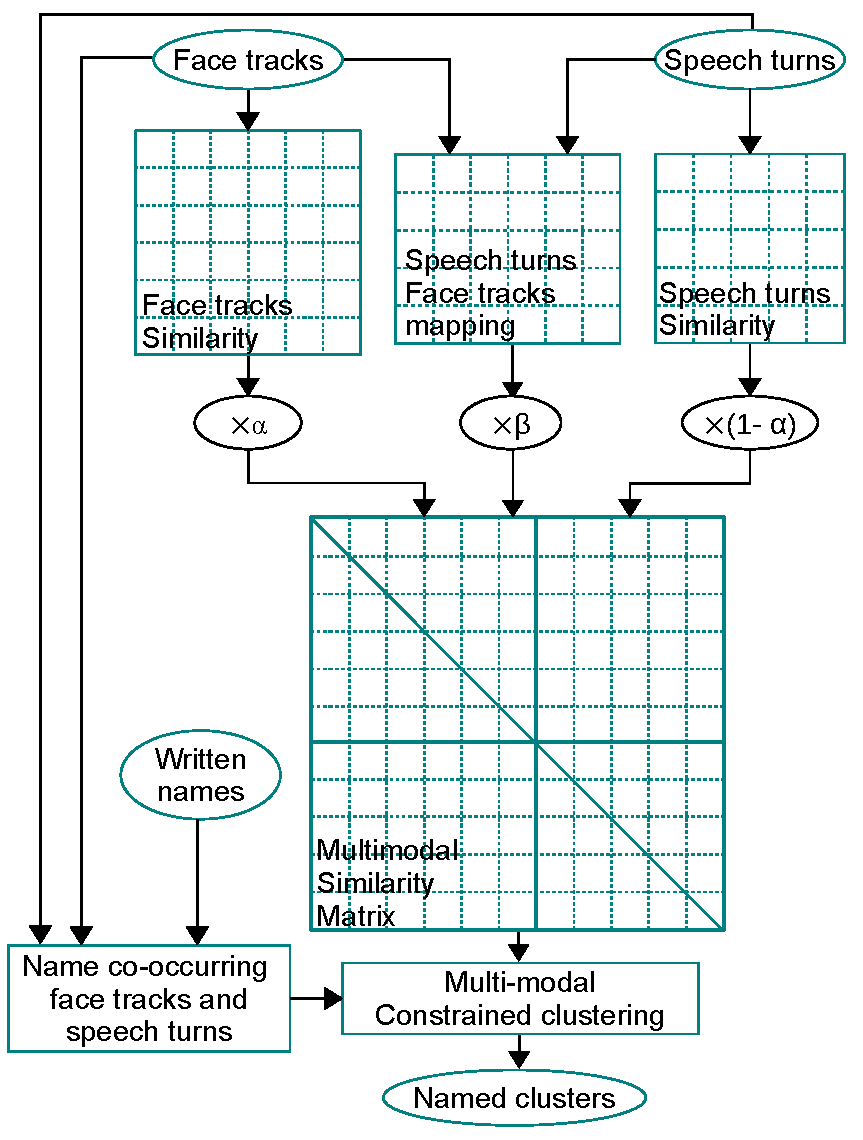
\includegraphics[width=0.9\linewidth]{figs/schema_clus_contraint.pdf}
 \caption {System overview}
 \label{fig:gene}
\end{figure}

For the image stream, after a face detection and tracking step, we find facial landmarks~\cite{URICAR--VISAPP--2012} and then compute an HoG descriptor on these points. These descriptors are projected using the LDML approach~\cite{GUILLAUMIN--IJCV--2012}. The similarity between two face tracks (normalized between 0 and 1) is based on the l2 distance between their descriptor.

In parallel we calculate a similarity between speech turns and co-occurring face tracks and complete this third matrix for those that do not co-occur via a transitive face track and speaker turn.

These three probability matrices are combined into a big multi-modal matrix using weights $\alpha$ and $\beta$ to give more or less importance to a modality. These parameters advance or delay the merge of components of a modality relative to others during the agglomerative clustering process. The goal of this clustering is to merge all face tracks / speaker turns of same person into a unique cluster. This clustering integrates the knowledge of written names to both identify clusters and also to prevent wrong merges (avoiding the fusion of clusters named differently). A complete description of this method can be found in~\cite{POIGNANT--MTAP--2015}.

For each identified cluster we list all shots (the shot segmentation was provided by the organizers) where they speak and appear on screen at the same time. A confidence score is computed for each (person, shot). This score is based on the temporal distance between the speaking face and its close written name. This confidence is equal to:

\begin{align*}
  confidence = & \left\{ 
  	\begin{array}{ll}
  		1/d  & \mbox{if the speaking face co-occur}  \\
  		 	 & \mbox{the written name}		\\
  		1+\delta &\mbox{otherwise}
  	\end{array} 
  \right.
\end{align*}

With $d$ the co-occurrence duration and $\delta$ the gap duration between the face track / speech turn and the written name.




\section{Results}

In table~\ref{tab:results} we detail the EwMAP, the MAP and the Correctness (noted C in the tables) (for these 3 metrics, higher is better, see~\cite{POIGNANT--MEDIAEVAL--2015} for more detail) obtained by the baseline and our system tune on an out domain corpus (for the first deadline: 01-jul-15) and tune on an in domain corpus (second deadline: 08-jul-15).

The baseline is a late propagation of written names onto speaker clusters (from a classical diarization) followed by a propagation of speaker names onto co-occurring speaking faces. This baseline don't take into account the similarity between face and does not benefit from the knowledge of written names during the diarization process. In addition to these 2 additional information, our method maximizes the stop criterion of the clustering based on the target metric (EwMAP) while the diarization of the baseline is perform to maximize the classical DER. 

\begin{table}[ht]
  \centering
  \begin{tabular}{|l|c|c|c|}
    \hline
	Run 											& EwMAP(\%)	& MAP(\%)	& C(\%) \\
	\hline
	\hline
	baseline~\cite{POIGNANT--INTERSPEECH--2012}	& 78.35		& 78.64		& 92.71		\\
	\hline
	limsi 01-jul-15 								& 83.13		& 83.46		& 93.19		\\
	limsi 08-jul-15 								& 84.56		& 84.89		& 94.11		\\
	\hline
	\hline
	Oracle propagation 							& \multirow{2}{*}{96.84}		& \multirow{2}{*}{96.84}		& \multirow{2}{*}{97.25}		\\
	mono-show									&			&			&			\\
	\hline
	Oracle propagation 							& \multirow{2}{*}{97.83}		& \multirow{2}{*}{97.83}		& \multirow{2}{*}{97.83}		\\
	cross-show 									&			&			&			\\
  	\hline
  \end{tabular}
  \caption{Results}
  \label{tab:results}
\end{table}

Two deadlines was proposed by the organizer, for the first one (1st july) we have tuned the $\alpha$, $\beta$ and the stop criterion of the clustering process on the dev set (out domain) and for the second deadline (8th july) we have tuned these parameters with the evaluation proposed via the leaderboard (computed on a sub-part of the test set). We can see a few improvement between the two tuning, shows that our method generalized well.

To determine the scope for further progress we used an oracle who propagate a written names (extract automatically) on a shot if the corresponding person speaking and appear in this shot. The propagation can be mono-show (meaning a written names appearing in a video can be only propagate to shots of the same video) or cross-show (all shots of the corpus can be tagged by a written name). For the moment our method used only a propagation mono-show, it is possible to earn up to 1\% of MAP with propagation cross-show.

In table~\ref{tab:precions_and_recall} we report the mean Precision and Recall over all queries. The high precision of our system made the choice of the confidence score (used to rank shots in the computation of the MAP) not really important. The tuning of the three parameters on a corpus in domain improve the recall about 1.3\% and decrease the precision about 0.8\%. In fact, the merge of speech turns together has been delayed relative to the merge of face tracks.

\begin{table}[ht]
  \centering
  \begin{tabular}{|l|c|c|}
    \hline
	Run 				& Precision(\%)	& Recall(\%)		\\
	\hline
	\hline
	limsi 01-jul-15 	& 98.5			& 82.9			\\
	limsi 08-jul-15 	& 97.7			& 84.2			\\
  	\hline
  \end{tabular}
  \caption{mean precision and recall}
  \label{tab:precions_and_recall}
\end{table}

In the next table (\ref{tab:errors}) we detail the numbers of queries 





\begin{table}[ht]
  \centering
  \begin{tabular}{|l|c|c|}
    \hline
			 											& 01-jul-15				& 08-jul-15				\\
	\hline
	\hline
	\#queries \textcircled{\tiny{0}}						& \multicolumn{2}{|c|}{2070}						\\

	\hline
	\textcircled{\tiny{0}} without any speaking 			& \multicolumn{2}{|c|}{\multirow{2}{*}{634}}		\\
	face in the reference \textcircled{\tiny{1}} 		& \multicolumn{2}{|c|}{} 						\\

	\hline
	\textcircled{\tiny{1}} where our system return		& \multirow{2}{*}{14}	& \multirow{2}{*}{15} 	\\
	at least 1 shot										&  						&						\\

	\hline
	\textcircled{\tiny{0}} with at least 1 speaking		& \multicolumn{2}{|c|}{\multirow{2}{*}{1436}}	\\
	face in the reference \textcircled{\tiny{2}}			& \multicolumn{2}{|c|}{} 						\\

	\hline
	\textcircled{\tiny{2}} with at least 1 correct shot	& \multirow{2}{*}{1251}	& \multirow{2}{*}{1267} 	\\
	return 												&  						&						\\
	
	\hline
	\textcircled{\tiny{2}} with all shots return wrong 	& 4						& 9				 		\\
	
	\hline
	\textcircled{\tiny{2}} with written names available 	& \multirow{2}{*}{137}	& \multirow{2}{*}{116} 	\\
	and no shot return 									&  						&						\\
	
	\hline
	\textcircled{\tiny{2}} without written names			& \multicolumn{2}{|c|}{44 (33 written names} 	\\
	available and neither shot return					& \multicolumn{2}{|c|}{with too many errors)} 	\\

  	\hline
  \end{tabular}
  \caption{Detail on results}
  \label{tab:errors}
\end{table}

From the 44 queries without written names available and neither shot return, 33 hypotheses corresponding to the queries have too many transcription errors to be mapped with the reference.

The 137 queries (01-jul-15) where a written name is available correspond to 648 shots in the reference. Only 214 of them were in a video where a written name is extracted, 434 of them need a cross-show propagation to be find (respectively 632, 199 and 433 for the second dead-line)


\section{Conclusion and future works}

This paper presented our approach and results at the MediaEval Person Discovery in Broadcast TV task. The process used an audio/video diarization constraint by written names on screen. 
This source of identities is used to both identify clusters and also to avoid wrong merge between cluster during the agglomerative clustering process.

For future works we will improve the distance between speech turns, try other clustering methods and cross-show propagation. 


\section{Acknowledgment}

This work was supported by the French National Agency for Research under grant ANR-12-CHRI-0006-01.
The open source CAMOMILE collaborative annotation platform\footnote{\url{http://github.com/camomile-project}} was used extensively throughout the progress of the task: from the run submission script to the automated leaderboard, including \emph{a posteriori} collaborative annotation of the test corpus.



% The following two commands are all you need in the
% initial runs of your .tex file to
% produce the bibliography for the citations in your paper.
\bibliographystyle{abbrv}
\bibliography{publi}  % sigproc.bib is the name of the Bibliography in this case
% You must have a proper ".bib" file
%  and remember to run:
% latex bibtex latex latex
% to resolve all references


\end{document}
